\section{Experiments}

	\begin{frame}
		\frametitle{Experiments Parameters}
		\begin{table}[H]
			\centering
			\begin{tabular}{|c|c|c|c|}
				\hline
				\rowcolor{tugreen}
				Parameter Description & Symbol & Value & Units\\
				\hline
				\rowcolor{tugreen!20}
				Diameter 							 & $d$ 					  & $0.5$ & \si[per-mode=symbol]{\meter}\\
				\rowcolor{tugreen!20}
				Weight 								 & $w$ 					  & $30$ &  \si[per-mode=symbol]{\kilogram}\\
				\rowcolor{tugreen!20}
				Linear Velocity Limit 			& $v_{max}$ 		  & $\ge 1.5$ &  \si[per-mode=symbol]{\meter \per \second}\\ 
				\rowcolor{tugreen!20}
				Linear Acceleration Limit    & $a_{max}$  		   & $1.0$ & \si[per-mode=symbol]{\meter \per \second \squared}\\
				\rowcolor{tugreen!20}
				Linear Deceleration Limit    & $a_{min}$  		   & $-2.5$ & \si[per-mode=symbol]{\meter \per \second \squared}\\
				\rowcolor{tugreen!20}
				Angular Velocity Limit 		  &$\omega_{max}$ & $3$ & \si[per-mode=symbol]{\radian \per \second}\\
				\rowcolor{tugreen!20}
				Angular Acceleration Limit & $\alpha_{max}$  & $3$ & \si[per-mode=symbol]{\radian \per \second \squared}\\
				\rowcolor{tugreen!20}
				Angular Deceleration Limit & $\alpha_{min}$  & $-3$ & \si[per-mode=symbol]{\radian \per \second \squared} \\
				\hline
			\end{tabular}
			\caption{The Robot Parameters}
		\end{table}
 	\end{frame}
 
	\begin{frame}
		\frametitle{Robot Specifications}
		\begin{figure}[hbtp]
			\centering
			\includegraphics[scale=0.6]{pictures/robotnik.pdf}
			\caption{NMPC Control Loop with Switching Objective}
		\end{figure}
	\end{frame}
 
	\begin{frame}
		\frametitle{Homogeneous Transformation}
		\begin{block}{Co-ordinate Transformation}
			\parbox[c][4\baselineskip][t]{\textwidth}{
			\[
				T_{obst\_map} = 
				T_{ft\_map}\enspace T_{r\_ft}\enspace T_{lsr\_r}
					\begin{pmatrix}
					x_{obst} \\
					y_{obst} \\
					z_{obst} \\
					1 
				\end{pmatrix}
			\]
			}
		\end{block}
		\begin{itemize}
			\item $
					T_{footprint\_map} \enspace \text{ }=
					\begin{pmatrix}
						\cos\theta_r & -\sin\theta_r & 0 & x_{r} \\
						\sin\theta_r & \cos\theta_r & 0 & y_{r} \\
						0 & 0 & 1 & 0 \\
						0 & 0 & 0 & 1 \\
					\end{pmatrix}
					$
			\item $
					T_{robot\_footprint} \enspace= 
					\begin{pmatrix}
						1 & 0 & 0 & 0 \\
						0 & 1 & 0 & 0 \\
						0 & 0 & 1 & -0.125 \\
						0 & 0 & 0 & 1 \\
					\end{pmatrix}
				$
			\item $
					T_{laser\_robot} \qquad= 
					\begin{pmatrix}
						1 & 0 & 0 & 0 \\
						0 & 1 & 0 & -0.245 \\
						0 & 0 & 1 & -0.051 \\
						0 & 0 & 0 & 1 \\
					\end{pmatrix}
				$
		\end{itemize}
	\end{frame}
 
	\begin{frame}
		\frametitle{Dynamic Obstacle Estimation}
		\begin{figure}[hbtp]
			\centering
			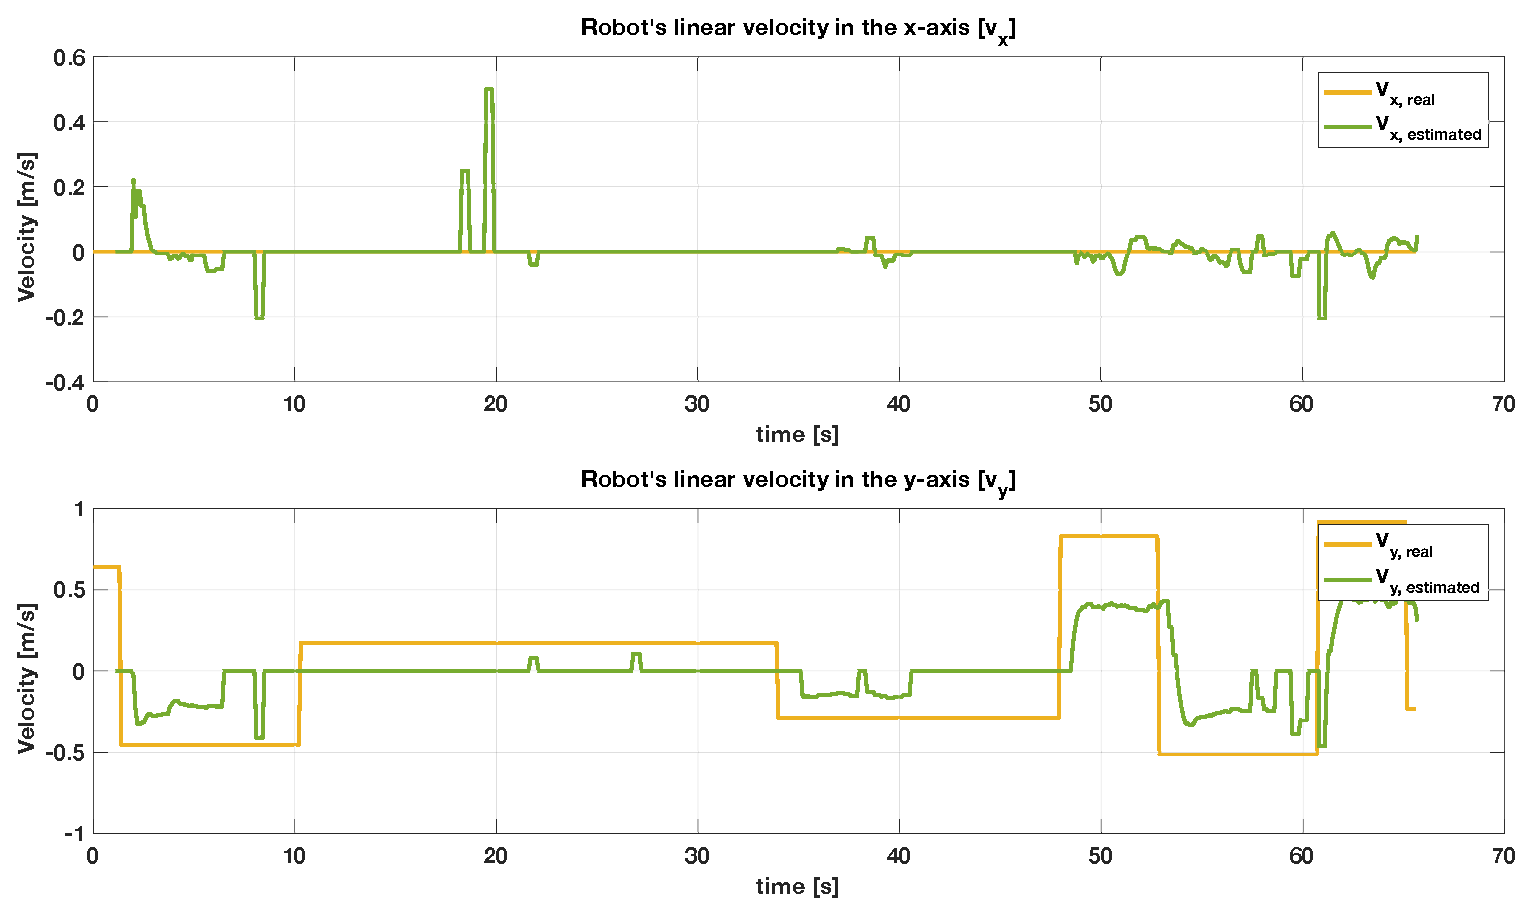
\includegraphics[scale=0.4]{pictures/estimate.eps}
			\caption{Velocities Estimations of Dynamic Obstacle}
		\end{figure}
	\end{frame}

	\begin{frame}
		\frametitle{Dynamic Obstacle Estimation}
		\centering
		\movie[width=0.9\textwidth, height=0.45\textwidth]
			{\includegraphics[width=0.9\textwidth]{pictures/kalman_filter_2.png}}{videos/kalman_filter_2.mov}
	\end{frame}
	
	\begin{frame}
		\frametitle{On-line Trajectory (prediction horizon)}
		\centering
		\movie[width=0.42\textwidth, height=0.45\textwidth]
			{\includegraphics[width=0.42\textwidth]{pictures/path.png}}{videos/path.mov}
	\end{frame}
	
	\begin{frame}
		\frametitle{Scenario I}
		\begin{figure}[hbtp]
			\centering
			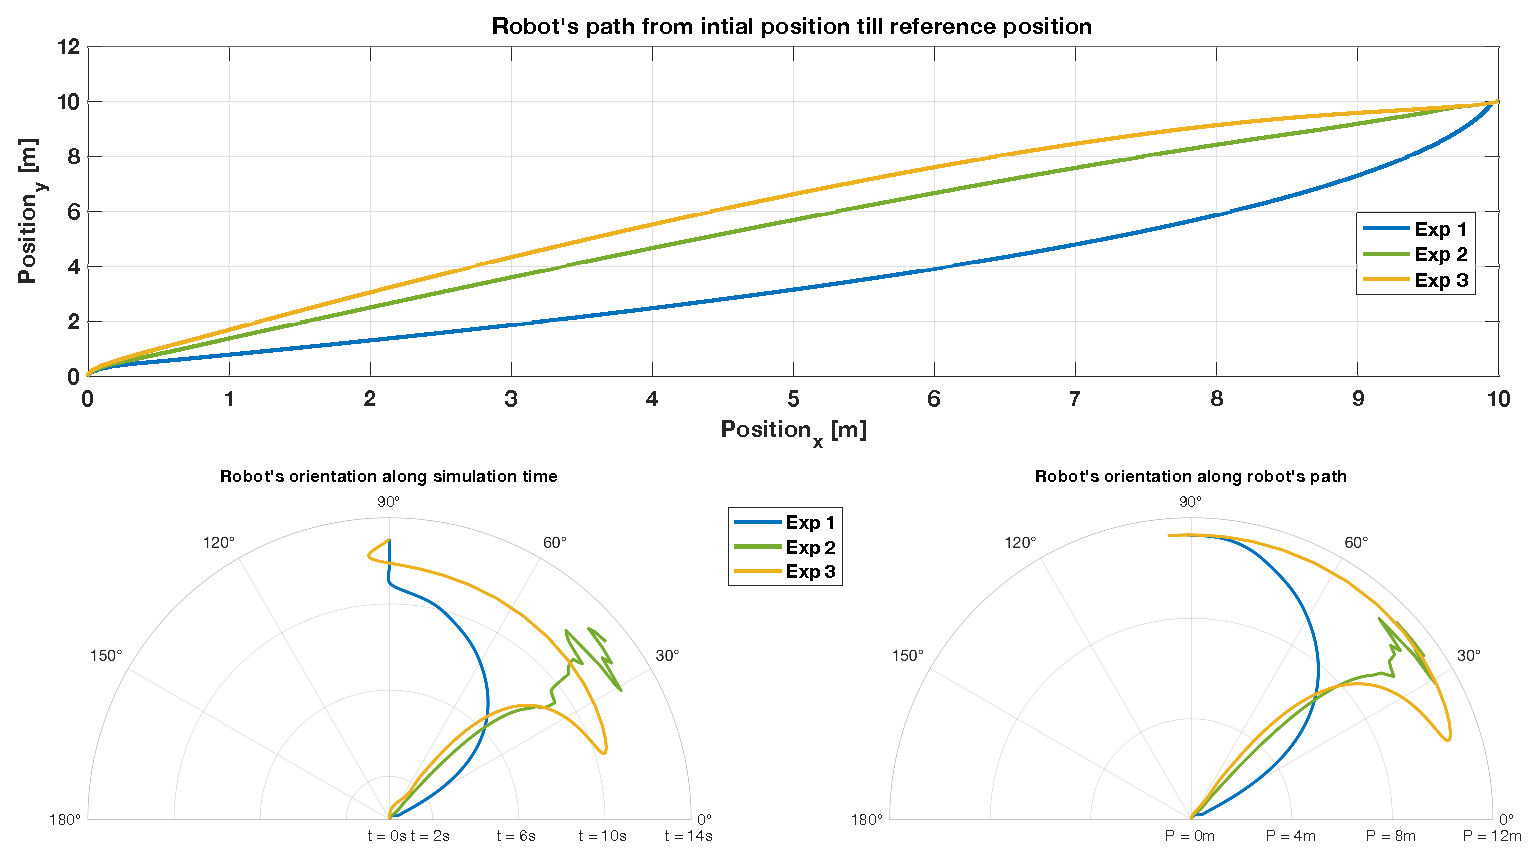
\includegraphics[scale=0.45]{pictures/graphs/sn1_states.eps}
			\caption{State Trajectory Evolution}
		\end{figure}
	\end{frame}

	\begin{frame}
		\frametitle{Scenario I}
		\begin{figure}[hbtp]
			\centering
			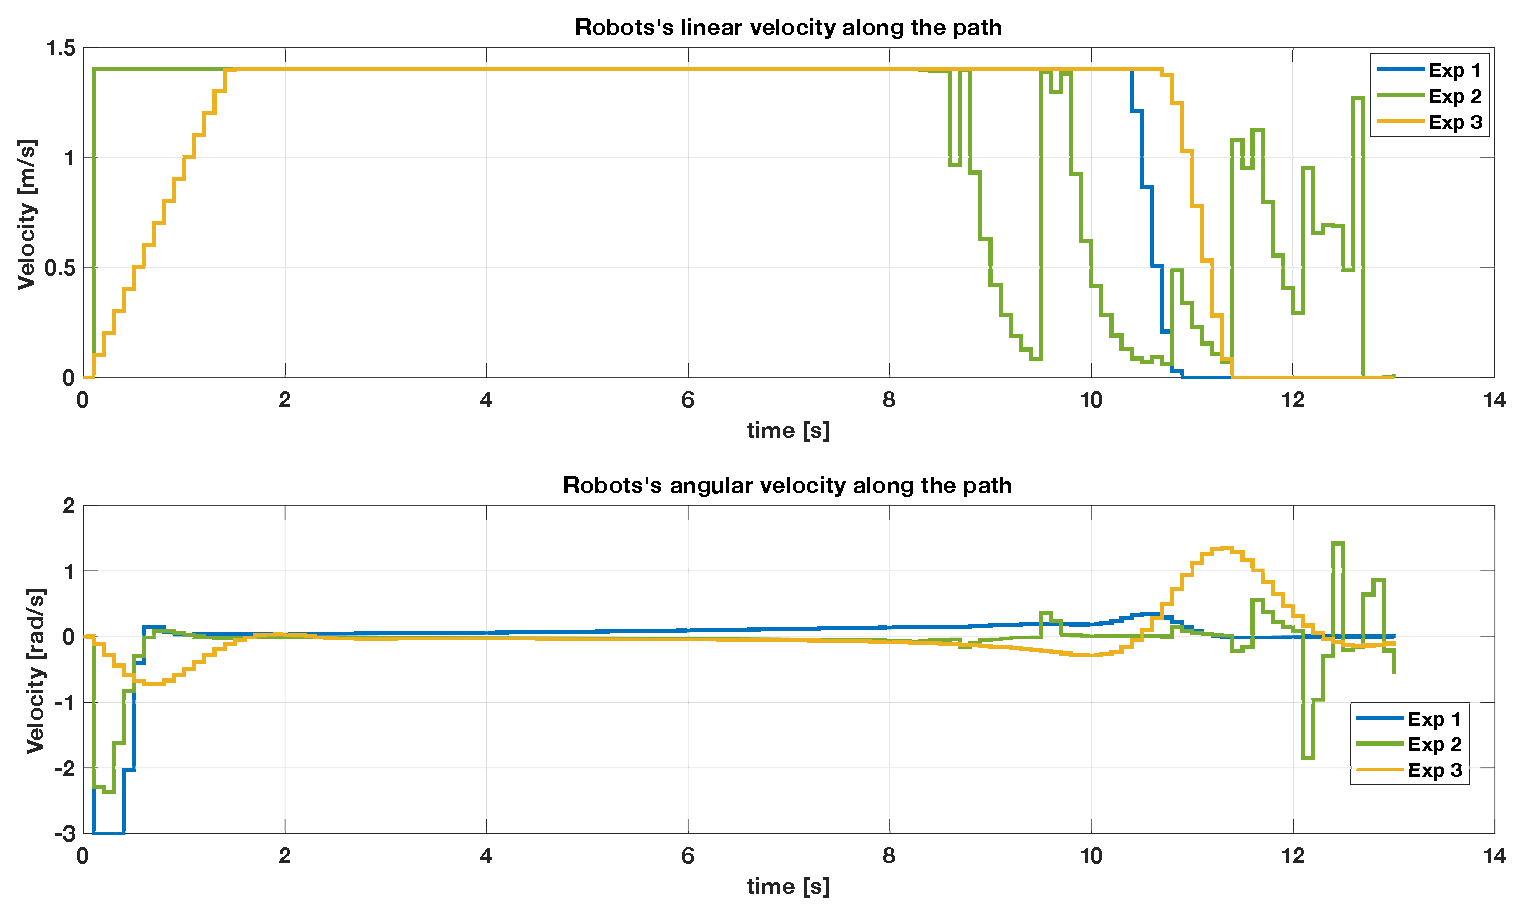
\includegraphics[scale=0.42]{pictures/graphs/sn1_inputs.eps}
			\caption{Input Trajectory Evolution}
		\end{figure}
	\end{frame}

	\begin{frame}
		\frametitle{Scenario I}
		\begin{figure}[hbtp]
			\centering
			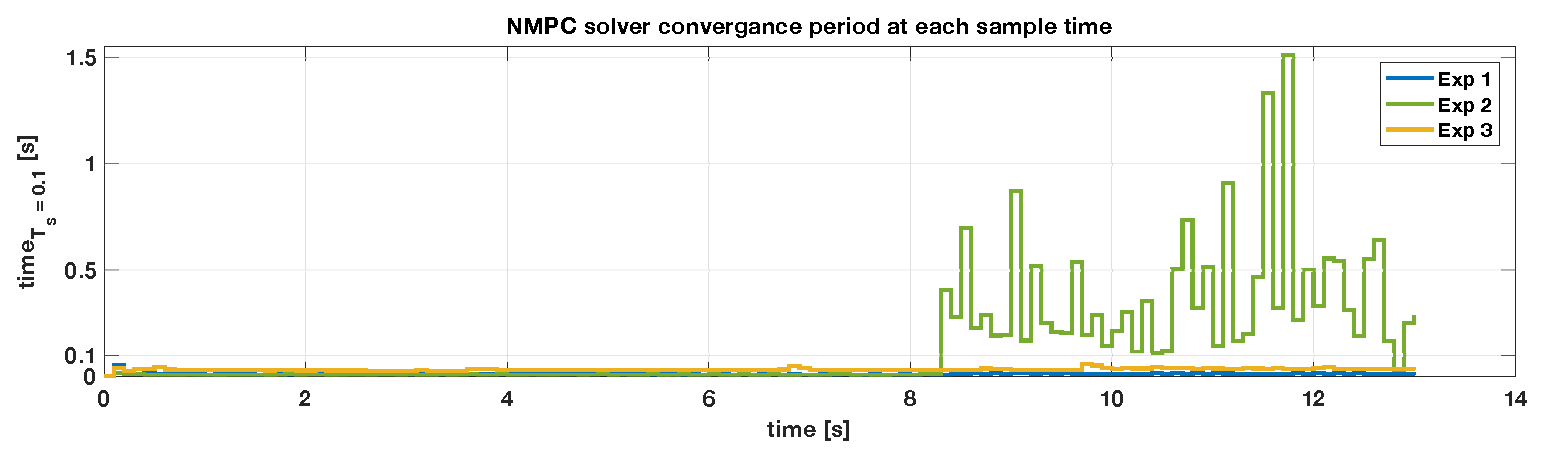
\includegraphics[scale=0.42]{pictures/graphs/sn1_solver_time.eps}
			\caption{NMPC Computational Effort}
		\end{figure}
	\end{frame}
 
 	\begin{frame}
 		\frametitle{Scenario II}
 		\begin{figure}[hbtp]
 			\centering
 			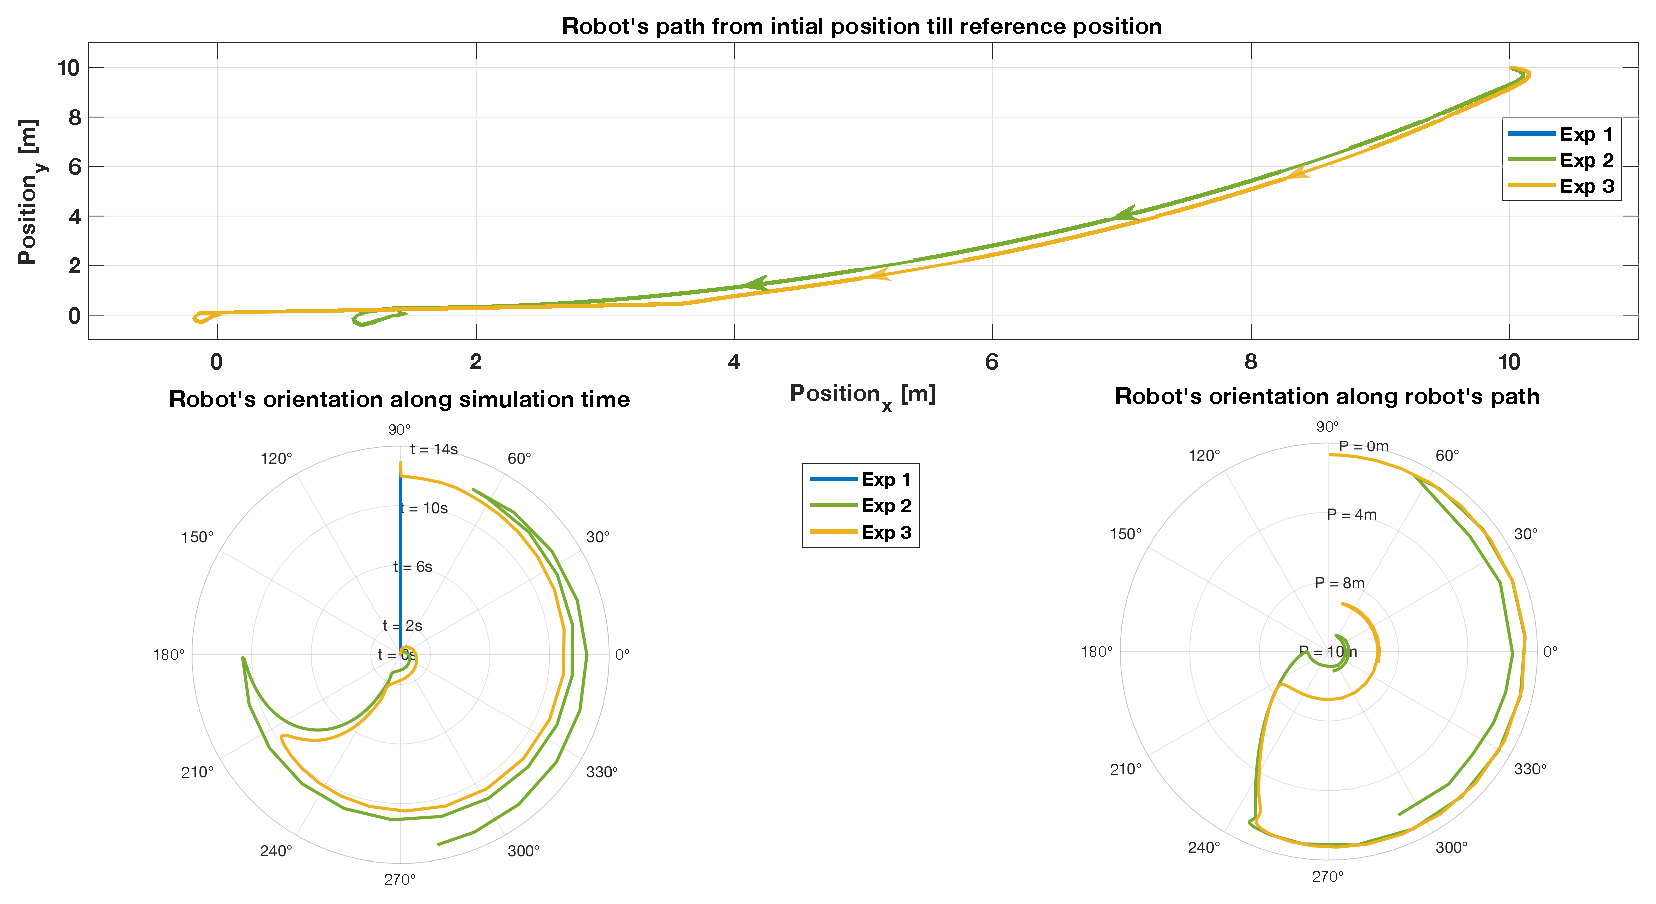
\includegraphics[scale=0.44]{pictures/graphs/sn1_states_2.eps}
 			\caption{State Trajectory Evolution}
 		\end{figure}
 	\end{frame}
 	
 	\begin{frame}
 		\frametitle{Scenario II}
 		\begin{figure}[hbtp]
 			\centering
 			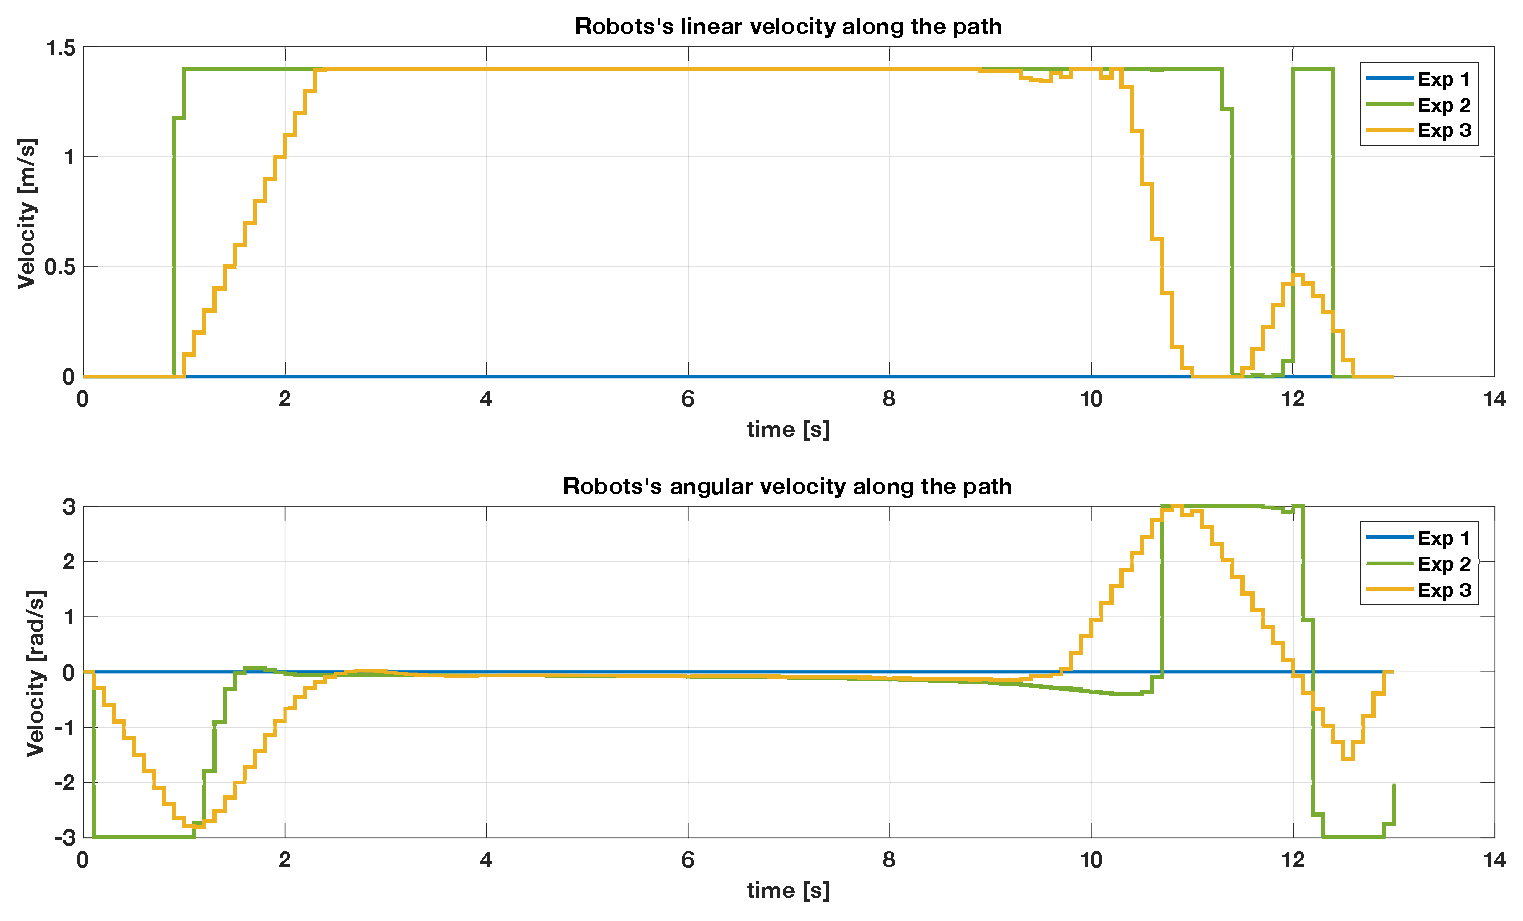
\includegraphics[scale=0.42]{pictures/graphs/sn1_inputs_2.eps}
 			\caption{Input Trajectory Evolution}
 		\end{figure}
 	\end{frame}
 	
 	\begin{frame}
 		\frametitle{Scenario II}
 		\begin{figure}[hbtp]
 			\centering
 			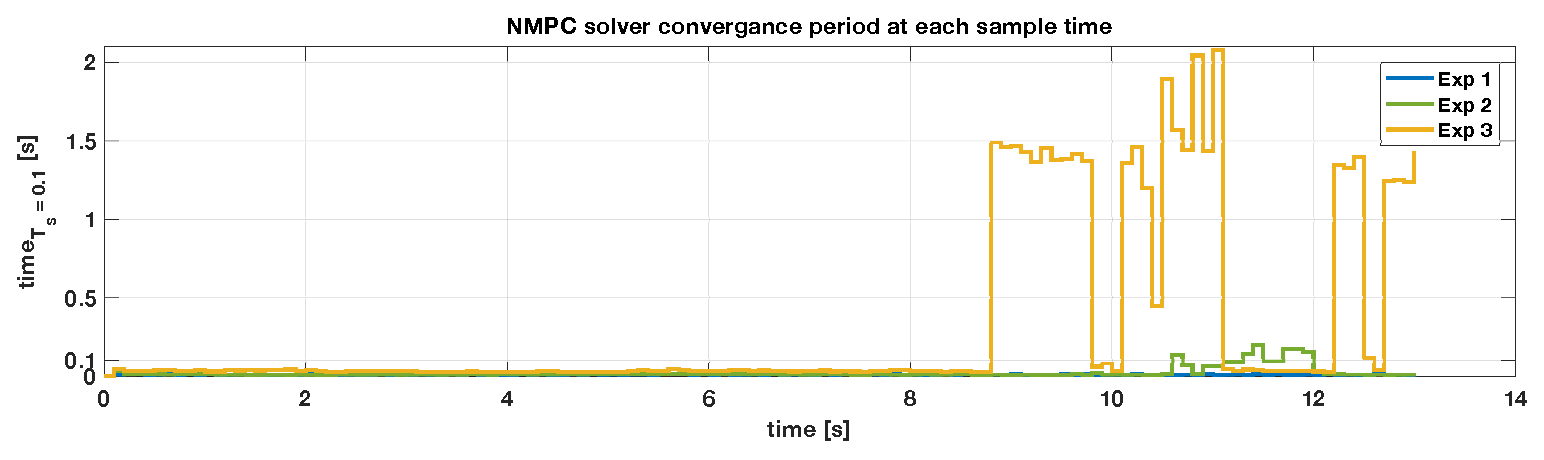
\includegraphics[scale=0.42]{pictures/graphs/sn1_solver_time_2.eps}
 			\caption{NMPC Computational Effort}
 		\end{figure}
 	\end{frame}
 	
 	\begin{frame}
 		\frametitle{Scenario III}
 		\begin{figure}[hbtp]
 			\centering
 			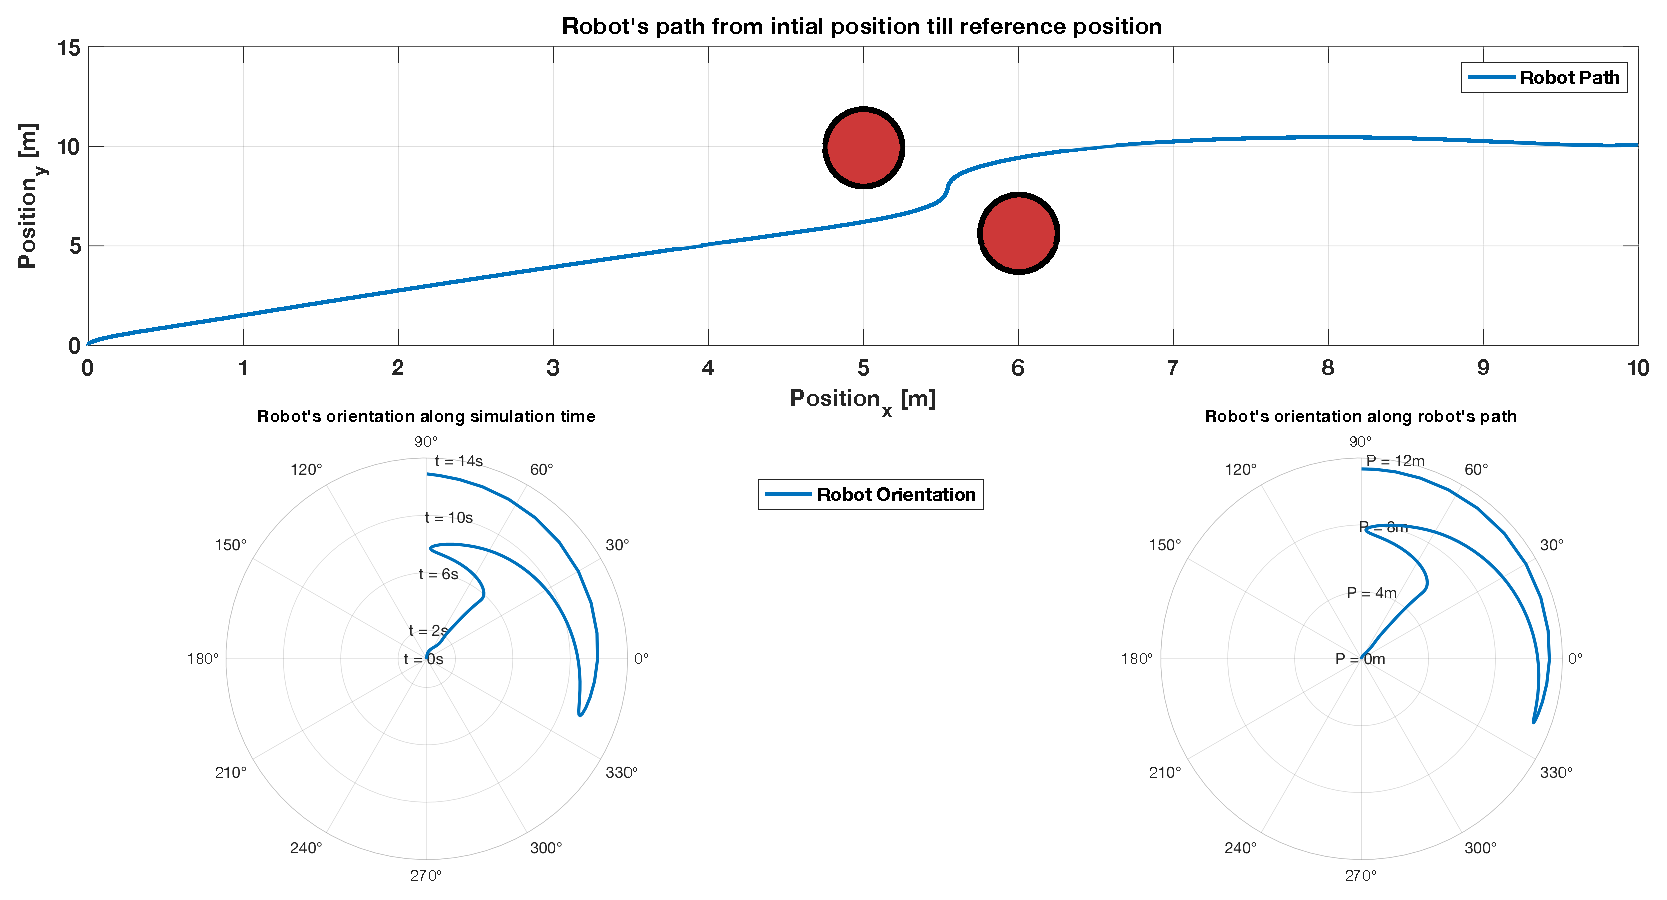
\includegraphics[scale=0.44]{pictures/graphs/sn2_states.eps}
 			\caption{State Trajectory Evolution}
 		\end{figure}
 	\end{frame}
 	
 	\begin{frame}
 		\frametitle{Scenario III}
 		\begin{figure}[hbtp]
 			\centering
 			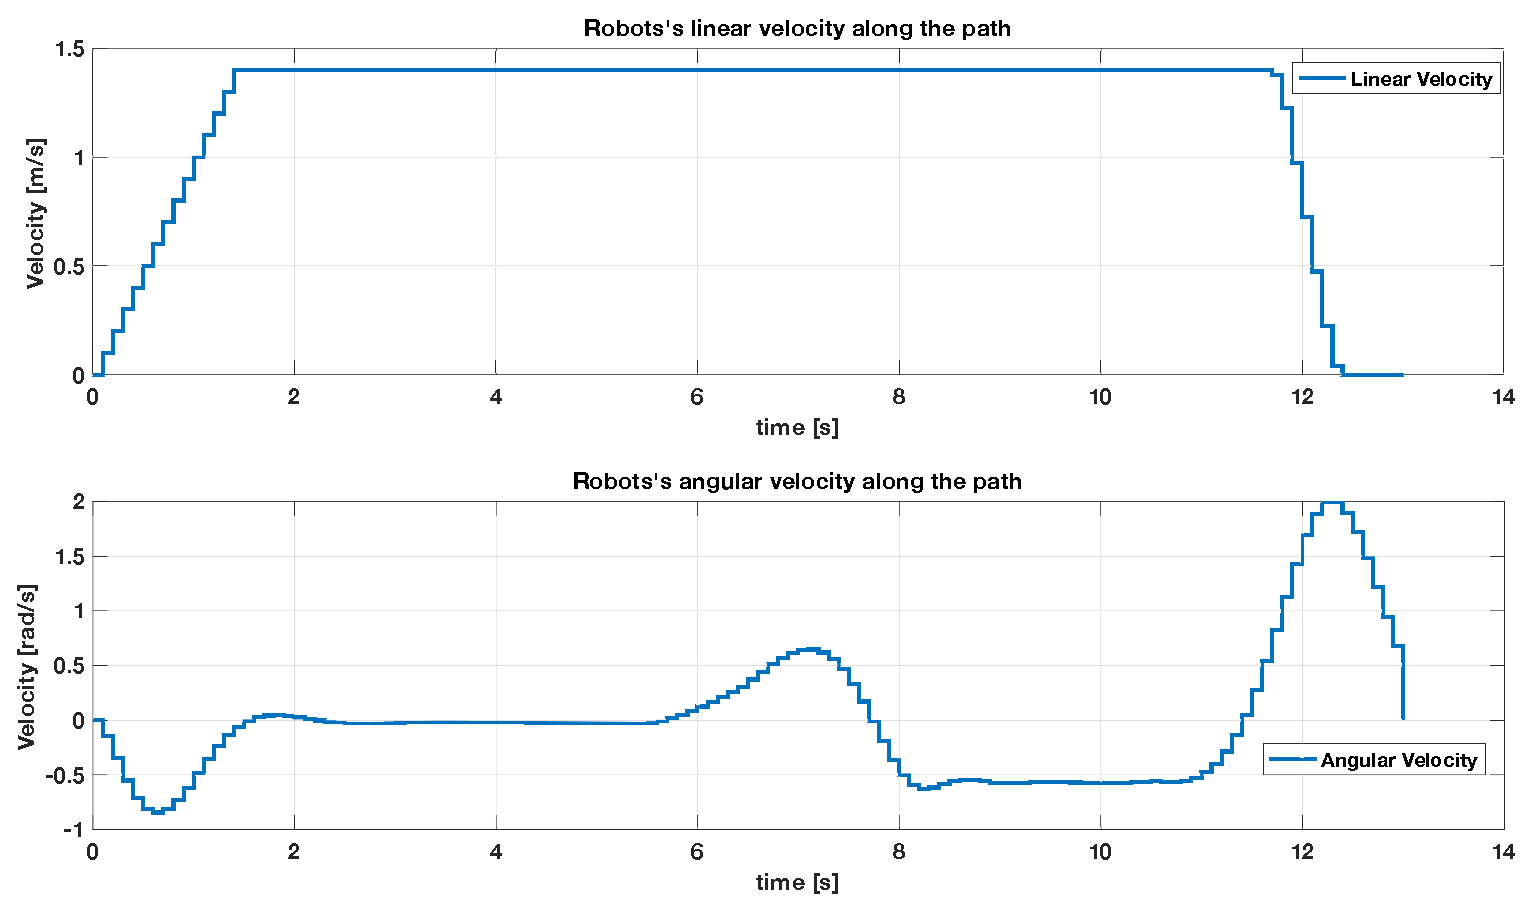
\includegraphics[scale=0.42]{pictures/graphs/sn2_inputs.eps}
 			\caption{Input Trajectory Evolution}
 		\end{figure}
 	\end{frame}
 	
 	\begin{frame}
 		\frametitle{Scenario III}
 		\begin{figure}[hbtp]
 			\centering
 			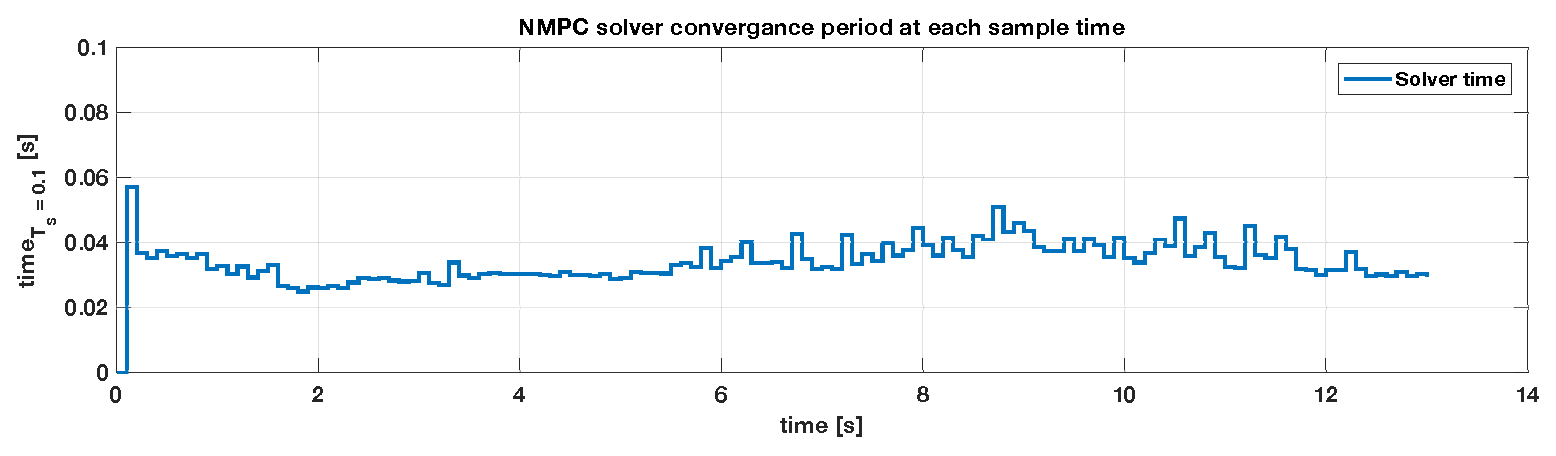
\includegraphics[scale=0.42]{pictures/graphs/sn2_solver_time.eps}
 			\caption{NMPC Computational Effort}
 		\end{figure}
 	\end{frame}
 
	\begin{frame}
		\frametitle{Scenario IV}
		\begin{figure}[hbtp]
			\centering
			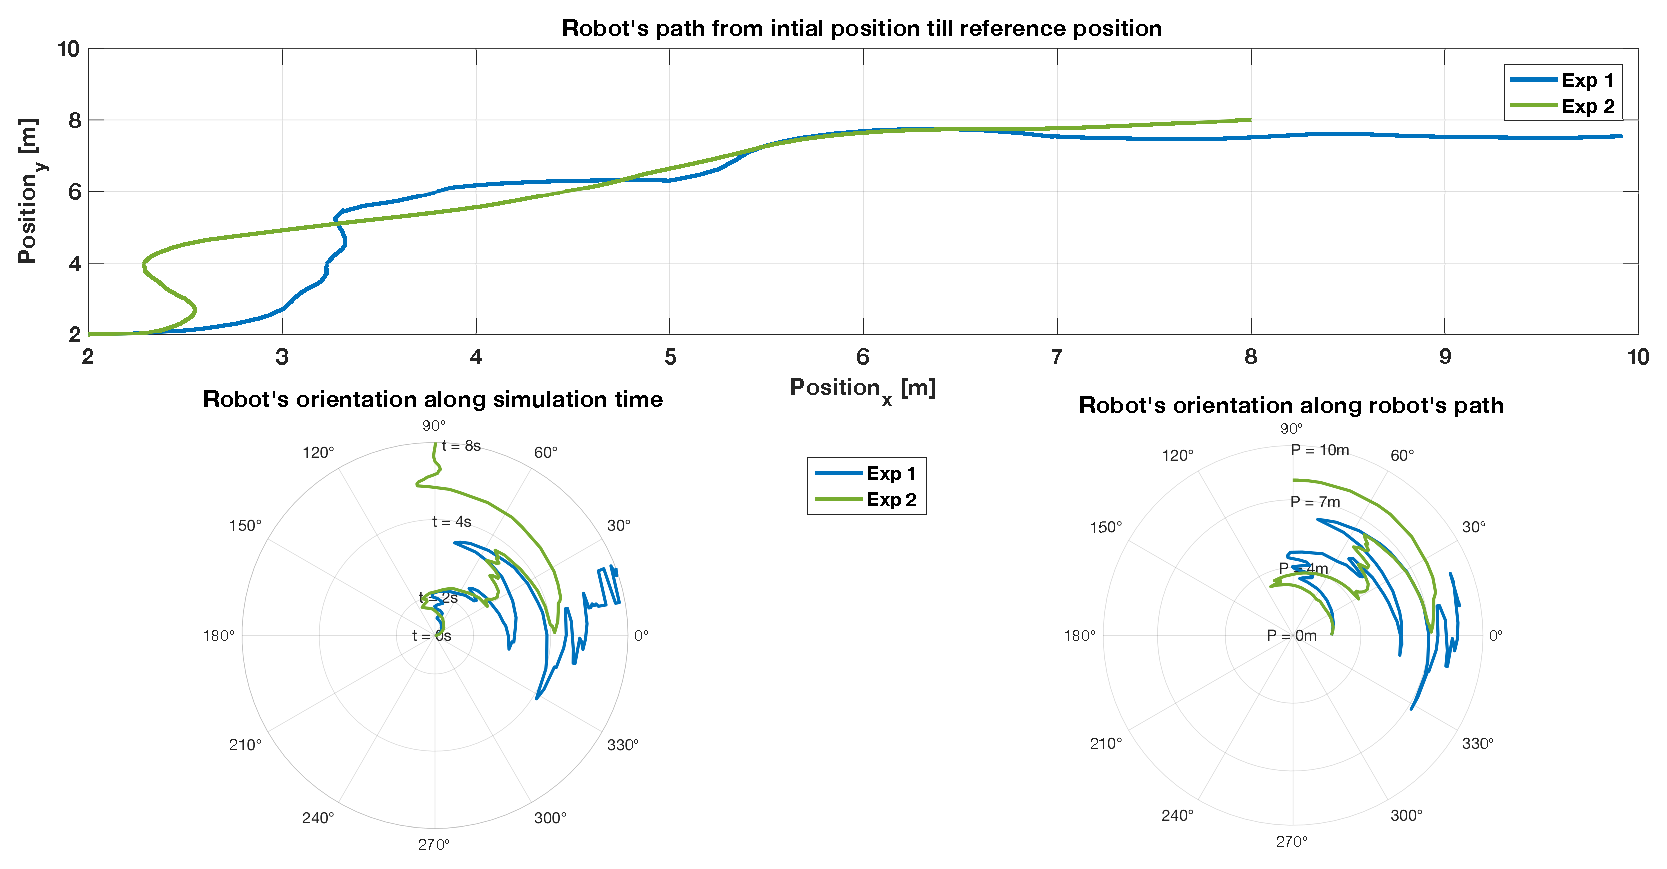
\includegraphics[scale=0.44]{pictures/graphs/sn3_states.eps}
			\caption{State Trajectory Evolution}
		\end{figure}
	\end{frame}
	
	\begin{frame}
		\frametitle{Scenario IV}
		\begin{figure}[hbtp]
			\centering
			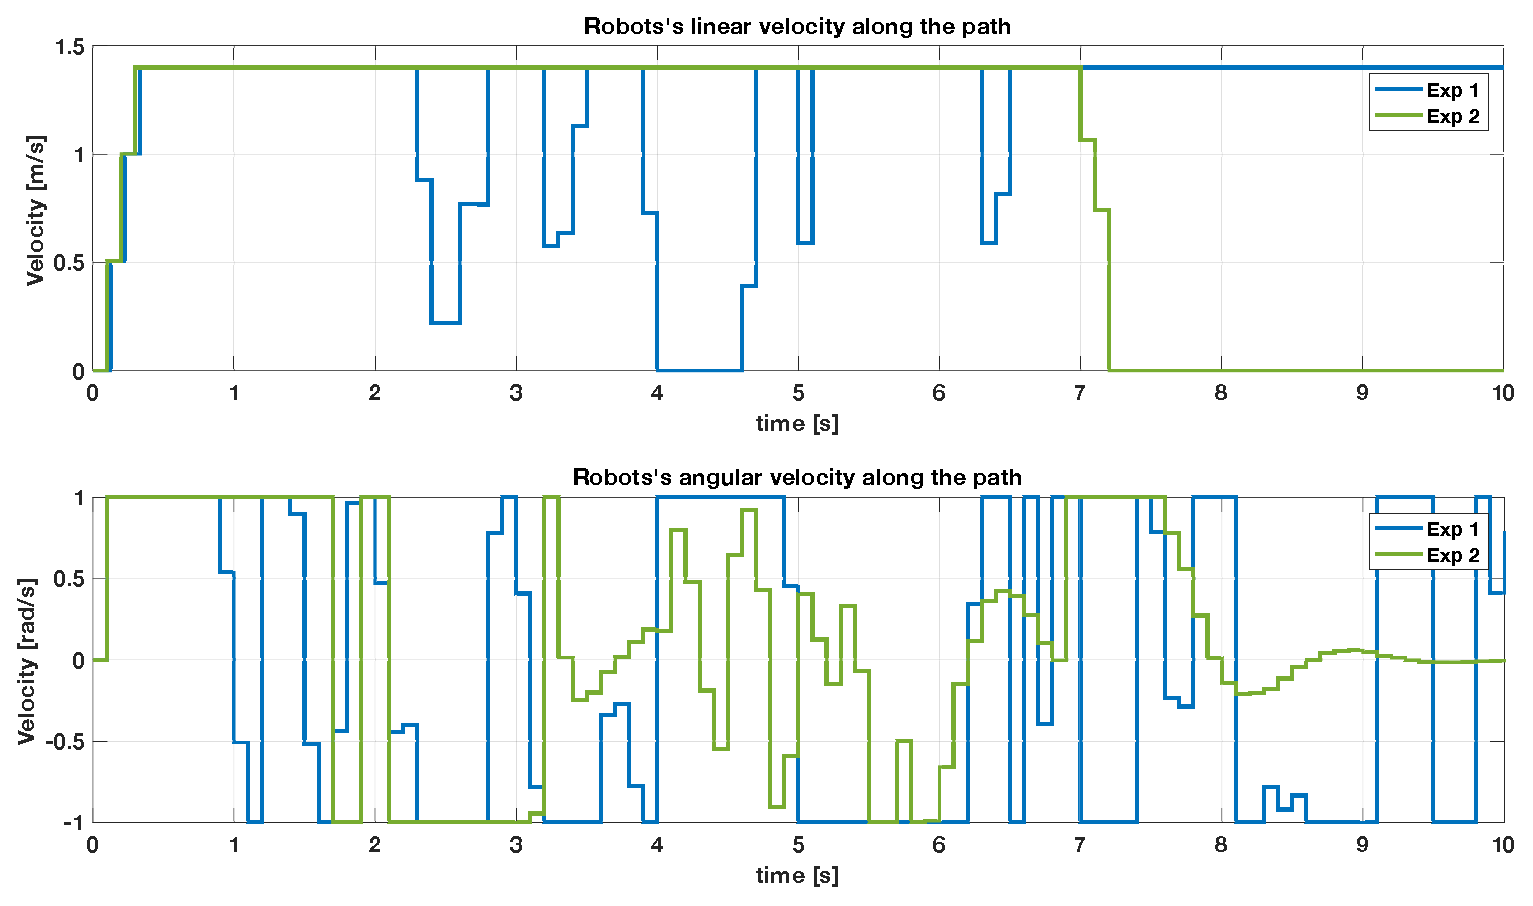
\includegraphics[scale=0.42]{pictures/graphs/sn3_inputs.eps}
			\caption{Input Trajectory Evolution}
		\end{figure}
	\end{frame}
	
	\begin{frame}
		\frametitle{Scenario IV}
		\begin{figure}[hbtp]
			\centering
			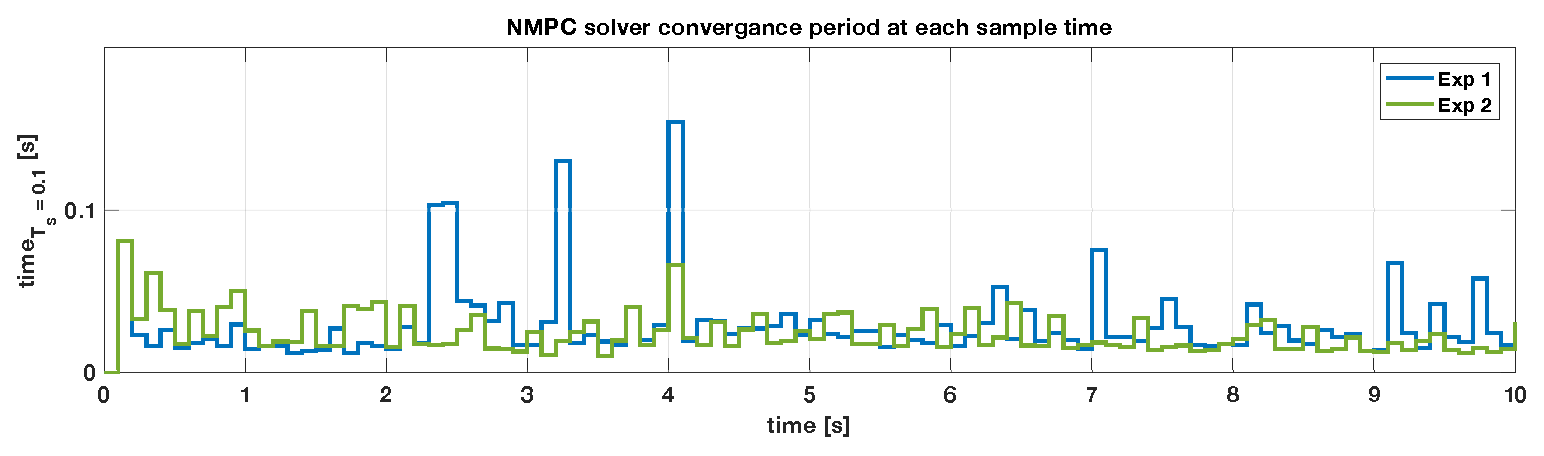
\includegraphics[scale=0.42]{pictures/graphs/sn3_solver_time.eps}
			\caption{NMPC Computational Effort}
		\end{figure}
	\end{frame}

	\begin{frame}
		\frametitle{Scenario IV}
		\centering
		\movie[width=0.451\textwidth, height=0.865\textheight]
		{\includegraphics[width=0.45\textwidth]{pictures/good_1.png}}{videos/good_1.mov}
		\nocite{hoy_matveev_savkin_2015}
	\end{frame}
